\documentclass[handout]{beamer}
%\documentclass{beamer}
\usetheme{Berlin}

\def\argmax{\mathop{\rm argmax}}
\def\argmin{\mathop{\rm argmin}}
\def\var{\mathop{\rm var}}
\def\cov{\mathop{\rm cov}}
\def\sign{\mathop{\rm sign}}
\def\X{\mathop{\bf X}}
\def\Y{\mathop{\bf Y}}
\def\Z{\mathop{\bf Z}}
\def\y{\mathop{\bf y}}
\def\x{\mathop{\bf x}}
\def\z{\mathop{\bf z}}
\def\W{\mathop{\bf W}}
\def\N{\mathop{\bf N}}
\def\S{\mathop{\bf S}}
\def\H{\mathop{\bf H}}
\def\I{\mathop{\bf I}}
\def\K{\mathop{\bf K}}
\def\L{\mathop{\bf L}}
\def\l{\mathop{\bf l}}
\def\f{\mathop{\bf f}}
\def\p{\mathop{\bf p}}
\usepackage{epsfig,amssymb,amsmath,enumerate,color,verbatim}
\usepackage{beamerthemesplit}
\usepackage{graphics}
\usepackage{graphicx}
\usepackage{hyperref}
\hypersetup{
    colorlinks=true,
    linkcolor=blue,
    filecolor=magenta,      
    urlcolor=cyan,
}



\newtheorem{ex}{Exercise}


\title[CART]{Lecture 6 Classification and regression trees : CART}
\author[Xiang Zhou]{%
  Xiang Zhou}
  \institute[City University of Hong Kong]{%
  Department of Mathematics \\
  City University of Hong Kong\\
  Based on the slides of Junhui Wang}

\date[\today]{ 2019}
\subject{Statistics}

\begin{document}

\frame {

\titlepage

}



%%%--------------------------------------------------------------------

\frame {

\frametitle{Tree structure}

\begin{itemize}

\item Tree method is the typical algorithm learning, more close to the viewpoint of computer science.
 No probabilistic model assumption is needed for the dataset.
 
 \item Will focus on classification tree, and extension to regression tree is direct.
\item Work as the weak classifier as the candidates for ensemble learning (such as boosting).
\item Reference: {\it Classification and Regression Trees} by L. Breiman, J. Friedman, R. Olshen, and C. Stone, Chapman $\&$ Hall, 1984

\item A medical example:
\begin{itemize}
\item Predict high risk patients who will not survive at least 30 days on the basis of the initial 24-hour data
\item 19 variables are measured during the first 24 hours. These include blood pressure, age, etc
\end{itemize}
\end{itemize}

}



%%%--------------------------------------------------------------------

\frame {

\frametitle{An example of tree structure}

\begin{figure}
\centering
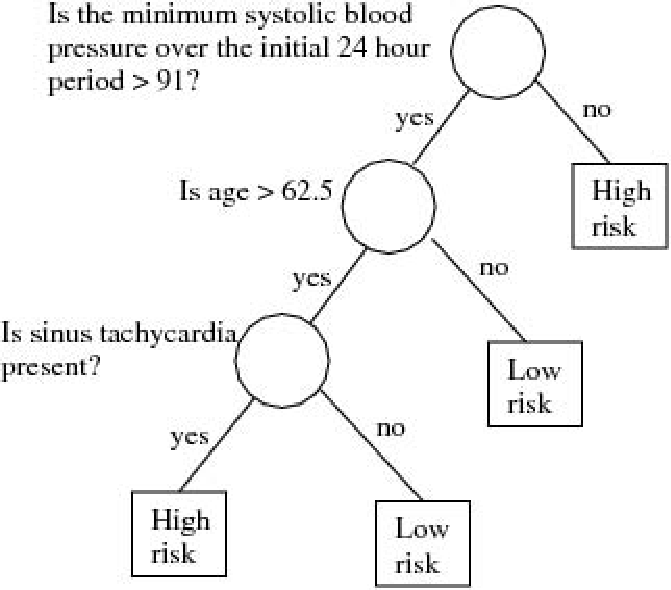
\includegraphics[width=3in]{Chp9_1.pdf}
\end{figure}

}

%%--------------------------------------------------------------------

\frame{
\frametitle{An example of  decision tree }

\begin{figure}
\centering
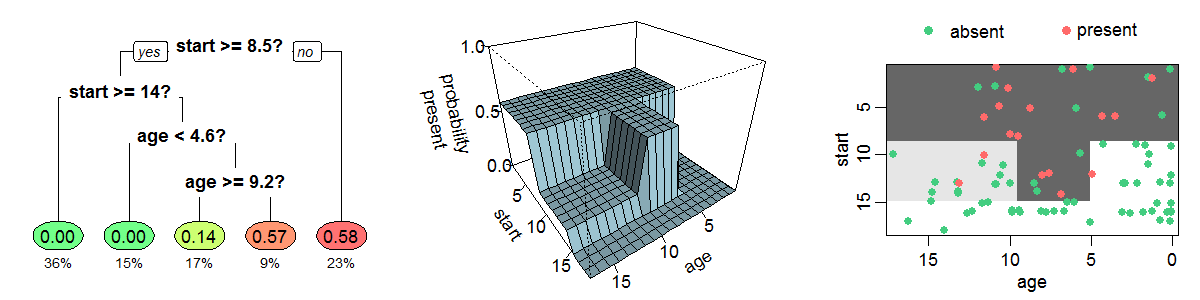
\includegraphics[width=0.99\textwidth]{Cart_tree_kyphosis.png}
\end{figure}
source: \href{https://en.wikipedia.org/wiki/Decision_tree_learning}
{wiki}
}



%%--------------------------------------------------------------------

\frame {

\frametitle{ }

Some notations:
\begin{itemize}
\item Denote the feature space by ${\cal X}$. The covariate $X=(X_1, X_2, \ldots, X_p)^T \in {\cal X} \subset {\cal R}^p$, some of which may be categorical.
\item 
${\cal Y}=\{ 1, \ldots, K\}$
\item Classification trees are constructed by repeated splits of subsets of ${\cal X}$ into two descendant subsets ${\cal X}={\cal X}_+\cup {\cal X}_- $, beginning with ${\cal X}$ itself --- recursive algorithm!
\item Definitions: 
{\bf node, terminal node (leaf node), parent node, child node, sibling node}
\item Two child nodes forms a partition of the region occupied by their parent node
\item Every leaf node is assigned with a class in $ \cal Y$.
\end{itemize}

}




%%%--------------------------------------------------------------------

\frame {

\frametitle{ }

\begin{itemize}
\item A node \footnote{ a subset of $\cal X$,  usually  in a rectangular form} is denoted by $t$
\item Its left child node is denoted by $t_L$ and right by $t_R$
\item The collection of all the nodes is denoted by $T$
\item The collection of all the leaf nodes by $\widetilde T \subset T$ 
\item A split is denoted by $s$, and the set of splits is denoted by ${\cal S}$
\end{itemize}

}



%%%--------------------------------------------------------------------

\frame {

\frametitle{ }

\begin{figure}
\centering
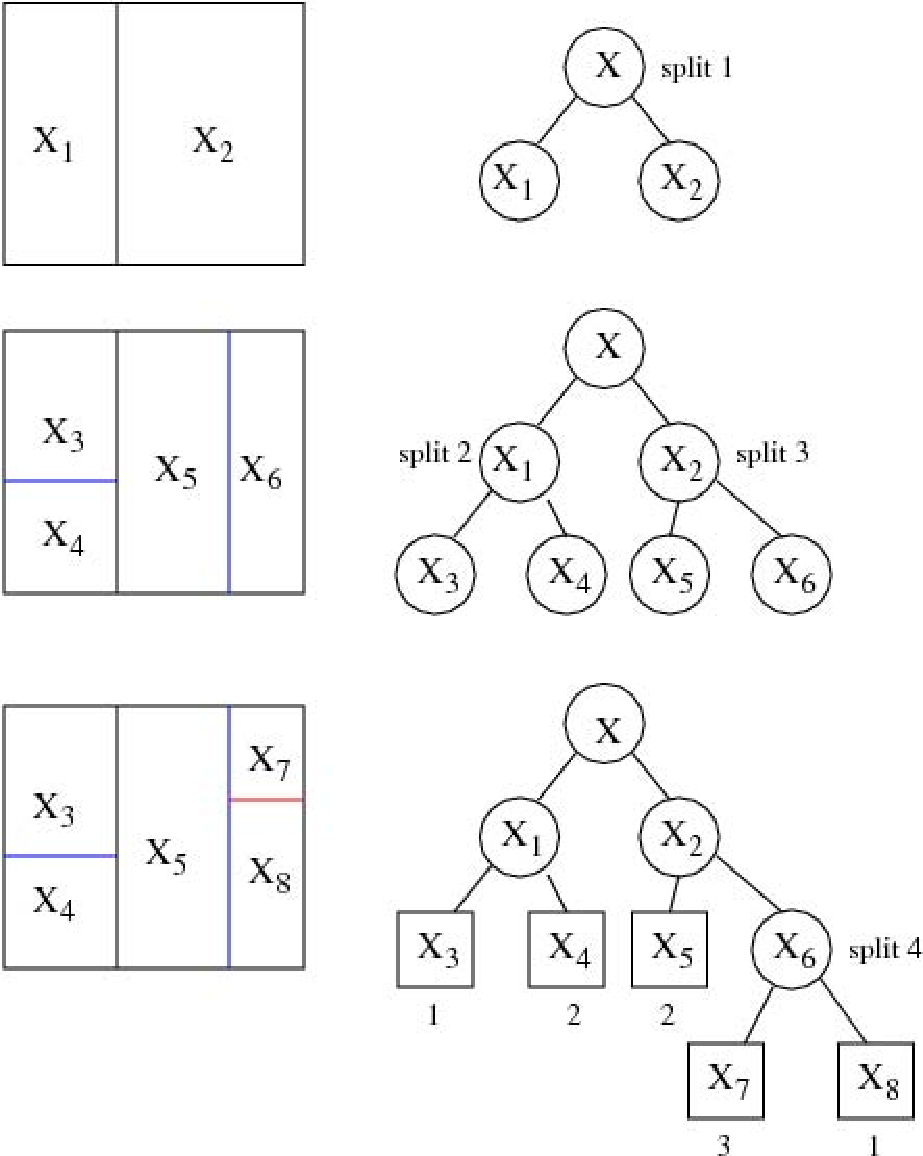
\includegraphics[width=0.8\textwidth, height=0.6\textwidth]{Chp9_2.pdf}
\end{figure}
 $X_i$ in the figure  refers to a subset of the input space $\cal X$.
 The collection of all leaf nodes, $\widetilde{T}$, is a partition of the   input space 
 $\cal X$.

}


%%%--------------------------------------------------------------------

\frame {

\frametitle{Key elements of a tree}

\begin{itemize}
\item The construction of a tree involves the following three elements:
\begin{enumerate}
\item when to split?   ~~The decisions when to declare a node terminal or to continue splitting it
\item how to split?   ~~The selection of the splits
\item Classifier on leaf ?  ~~The assignment of each terminal node to a class
\end{enumerate}
\item In particular,  
\begin{enumerate}
\item (how to split ? ) A set of binary questions used as splits (``{\texttt if ... else ... }'')
\item (which specific split is preferred ?)  A goodness of split criterion $\phi(s, t)$ that can be evaluated for any split $s$ of any node $t$
\item (when to stop split?) A stop-splitting rule
\item (classifier? ) A rule for assigning every terminal node to a class
\end{enumerate}
\end{itemize}

}



%%%--------------------------------------------------------------------

\frame {

\frametitle{Standard set of questions}

\begin{itemize}
\item Each split depends on the value of only a unique variable
(one component/feature of the input vector $X$)
\item For each variable $X_j$, ${\cal S}$ includes all questions of the form
$$
\{ \mbox{Is $X_j \in A$?} \} 
$$
\vspace{-6mm}
\begin{itemize}
\item If $X_j$ is continuous or ordinal, $A=(-\infty,c]$
\item If $X_j$ is categorical, $A$ is a subset of categories
\end{itemize}
\item The splits for all $p$ variables constitute the standard set of questions
\end{itemize}

}


%%%--------------------------------------------------------------------

\frame {

\frametitle{Goodness of splits}

\begin{itemize}
\item The goodness of split is measured by an {\bf impurity} function defined for each node
\item Intuitively, we want each leaf node to be ``pure", that is, one class dominates
and then assignment to this dominant class would have a minimal misclassification rate:
\vspace{0.3cm}
\begin{figure}
\centering
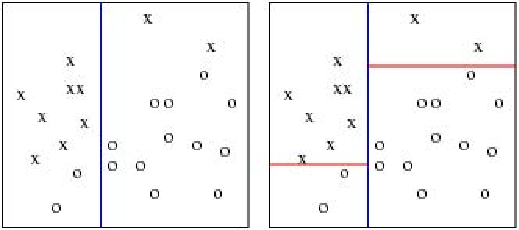
\includegraphics[width=3in]{Chp9_3.pdf}
\end{figure}
\end{itemize}

}



%%%--------------------------------------------------------------------

\frame {

\frametitle{The node impurity function}

Define the empirical distribution inside the node $t$:
$$ p_{tk}=|t|^{-1} \sum_{x_i \in t} I(y_i = k)\approx \Pr(Y=k| X\in t), ~~k =1,\ldots, K$$
``Purity'' means $p_{tk}$ is independent of $k$.
The  possible {\bf impurity functions} 
\footnote{ a {\bf larger } value means more impure, less pure.} $i(t)$  of the node $t$ are
\begin{itemize}
\item Misclassification error: $\displaystyle 1-\max_{1 \le k  \le K} p_{tk}$
\item Gini index: $\sum_k  p_{tk}(1-p_{tk}) = 1 - \sum_k p_{tk}^2$
\item (Cross) entropy: $-\sum_k p_{tk} \log p_{tk}$
\end{itemize}
}

\begin{frame}
For the two classes, write  the binary distribution vector $p_{t}=(p,1-p)$, then  
\begin{itemize}
\item Misclassification error: $1-\max(p,1-p)$
\item Gini index: $2p(1-p)$
\item (Cross) entropy: $-p\log p - (1-p)\log(1-p)$
\end{itemize}

\begin{center}
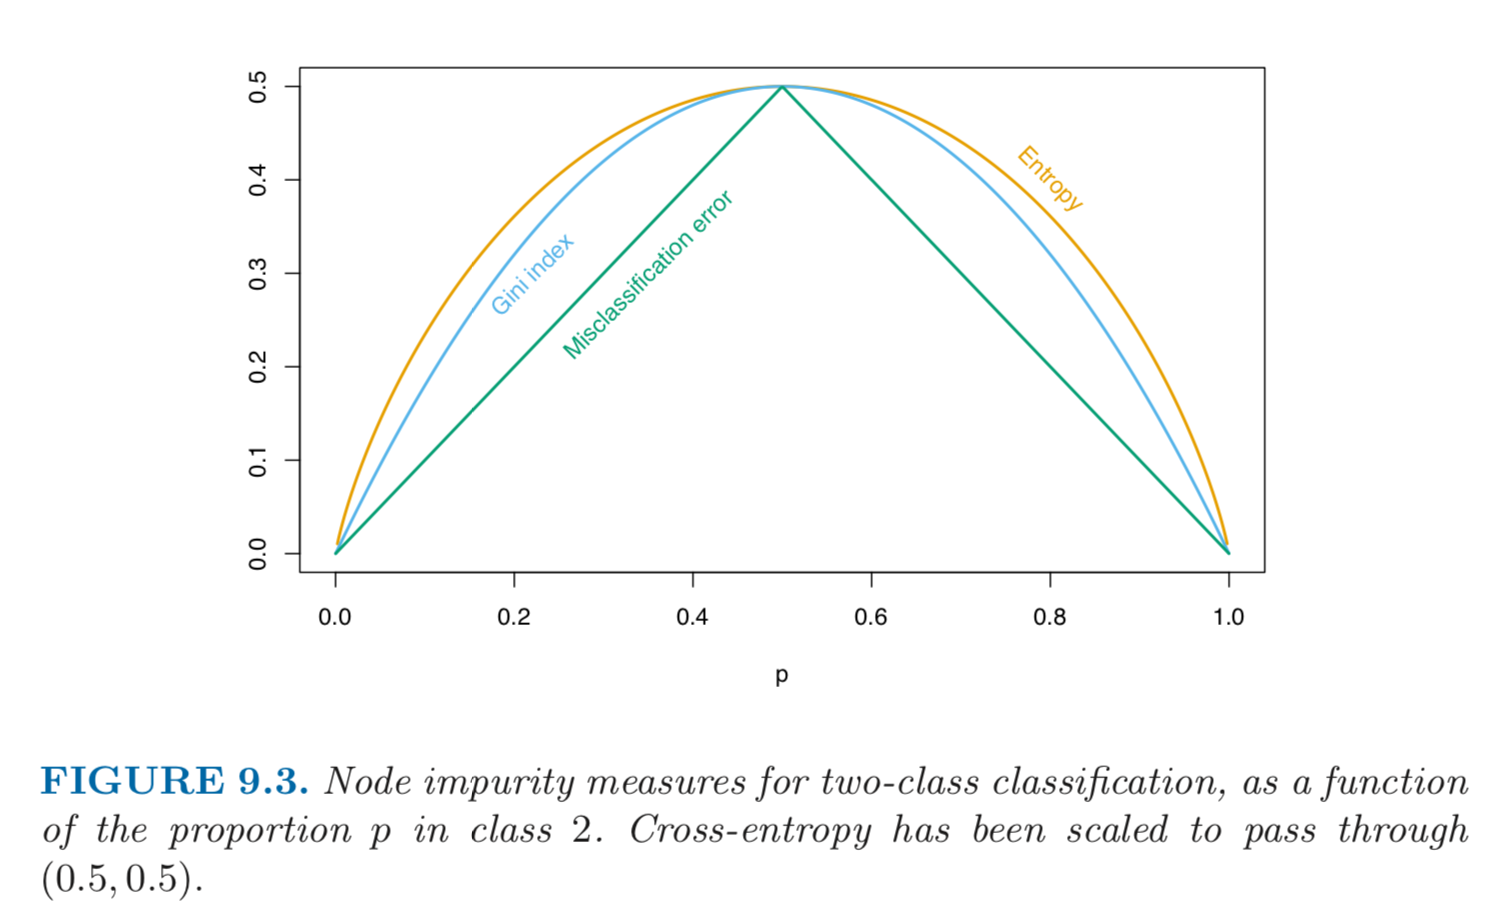
\includegraphics[width=0.8\textwidth]{impurity-binary.png}
\end{center}

\end{frame}



%%%--------------------------------------------------------------------

\begin{frame}
\begin{ex}
Assume $p=(p_1,\ldots, p_K)$ is the distribution of a random variable :  $p_k =\Pr(Y=k)$.
Solving the following optimization problem subject to the constraint
$\sum_k p_k =1 $ and $p_k \in [0,1]$ for all $k$:
\begin{enumerate}
\item (entropy) $\max_p ( \mbox{ or } \min_p )~  -\sum_k p_k \log p_k $
\item (Gini) $\max_p  (\mbox{ or }  \min_p) ~ \sum_k p_k (1-p_k)$
\end{enumerate}
\end{ex}
\end{frame}

%%%--------------------------------------------------------------------

\begin{frame}
\begin{ex}
To see the above form of the misclassification error,
consider the Bayes classifier:
$x\in t \to  k^*(x)=\argmax_k p_{k}$.
Show that the misclassification rate of this classifier 
$
|t|^{-1} \sum_{x_i \in t}  I ( y_i \neq k^*(x_i))
$
equals   $1- \max_{k} p_{k}$.
(we left out $t$ in $p_{tk}$)
\end{ex}
\begin{ex}
To see the Gini index, 
consider the Gibbs classifier: assign 
$x\to G(x)= k$ with probability $p_{k}$. 
Show that the training error rate of this Gibbs classifier 
\[
|t|^{-1} \sum_{x_i\in t}  I ( y_i \neq G(x_i))
\]
equals    $\sum_{k\neq k'} p_k p_{k'}=\sum_{k} p_k (1-p_k)$.
\end{ex}

\end{frame}
%%%--------------------------------------------------------------------


\frame{{Goodness of split}

\begin{itemize}
\item
A split $s$ means  that $t$ is partitioned into $t=t_L \cup t_R$.
\item Its {\bf goodness} is measured by 
 $$\boxed{
 \phi(s,t) = i(t) - p_L i(t_L) - p_R i(t_R)},$$ where $p_L= |t_L|/ |t|$ and $p_R=|t_R|/|t|$ are proportions of the samples in node $t$ that go to the left child $t_L$ and the right child of $t_R$, respectively.
 \item  Search the optimal split $s$ with the largest value of goodness from all possible split $\cal S$, i.e.,
 \[ \argmin_{s\in {\cal S}}  ~~ \{ p_L i(t_L) + p_R i(t_R)\}\]
\end{itemize}
}
\begin{frame}
\begin{ex}
Consider a node has two classes with 400 observations in each class,
denoted by $(400+, 400-)$. Compute the goodness of split
corresponding to the above three impurity functions for the following two kinds of split
\begin{enumerate}
\item 
one child node contains $(300+,100-)$ and the other contains $(100+,300-)$.
\item 
one child node contains $(200+,400-)$ and the other contains $(200+,0-)$.
\end{enumerate}
explain your result.
\end{ex}
\end{frame}

\begin{frame}
\begin{ex}
Show that the goodness $\phi(s,t)$ is always non-negative for the misclassification error impurity function.
i.e., the mis-classficiation error always increases after splitting.
What about the other two choices of impurity functions.
\end{ex}

\end{frame}



%%%--------------------------------------------------------------------

\frame {

\frametitle{Stopping criteria}

\begin{itemize}
\item A simple criteria: stop splitting a node $t$ when
$$
\max_{s \in {\cal S}} \frac{|t|}{n} \phi(s,t) < \beta,
$$
where $\beta$ is a pre-specified threshold
\item The idea is to stop splitting when the node is sufficiently pure or sufficiently small
\item The above stopping criteria may not work well; other more sophisticated stopping rules have been proposed
\end{itemize}

}



%%%--------------------------------------------------------------------

\frame {

\frametitle{Class assignment rule}

\begin{itemize}
\item A class assignment rule assigns a class $k = \{1, \ldots,K\}$ to every terminal node $t \in \widetilde T$
\item The class assigned to node $t \in \widetilde T$ is denoted by $\kappa(t)$
\item For 0-1 loss, the class assignment rule is the Bayes rule
$$
\kappa(t)=\argmax_k~  p_{tk}
$$
the dominant class inside the leaf node.
\end{itemize}

}



%%%--------------------------------------------------------------------

\frame {

\frametitle{Extension to regression}

\begin{itemize}
\item ${\cal S}$ remains the same
\item Impurity function is replaced
by the variance : $i(t)=\sum_{i \in t} (y_i - \mbox{avg}(y|t))^2$
\item Goodness of fit means the reduction 
of the variance: $\phi(s,t)=i(t)-i(t_L)-i(t_R)$
\item Stopping rule remains the same
\item Response assignment rule: $\kappa(t)=\mbox{avg}(y|t)$
\end{itemize}

}



%%%--------------------------------------------------------------------

\frame {
{Personal Remark }
The tree splitting method is quite similar to 
one of the most important adaptive computational methods in
traditional  the numerical methods for PDE:
\href{https://en.wikipedia.org/wiki/Adaptive_mesh_refinement}
{adaptive mesh refinement (AMR)} 

Indeed, the implement of AMR uses the tree data structure for fast processing.

\bigskip
The impurity function in tree classification
is like the monitor function (the simplest form
is the magnitude of the solution's gradient ) 
in AMR.

There are lots of similarities of adaptivity ideas
in machine learning and computational maths,
which is now under the fast advancement in research works.
}


%%%--------------------------------------------------------------------

\frame {

\frametitle{Example: Digit recognition example}

\begin{itemize}
\item The 10 digits are shown by different on-off combinations of seven horizontal and vertical lights
\item Each digit can be represented by a 7-dimensional vector of zeros and ones. The $i$-th sample is $x_i = (x_{i1}, \ldots, x_{i7})$. If $x_{ij} = 1$, the $j$-th light is on, and vice versa
\end{itemize}

\vspace{0.3cm}
\begin{figure}
\centering
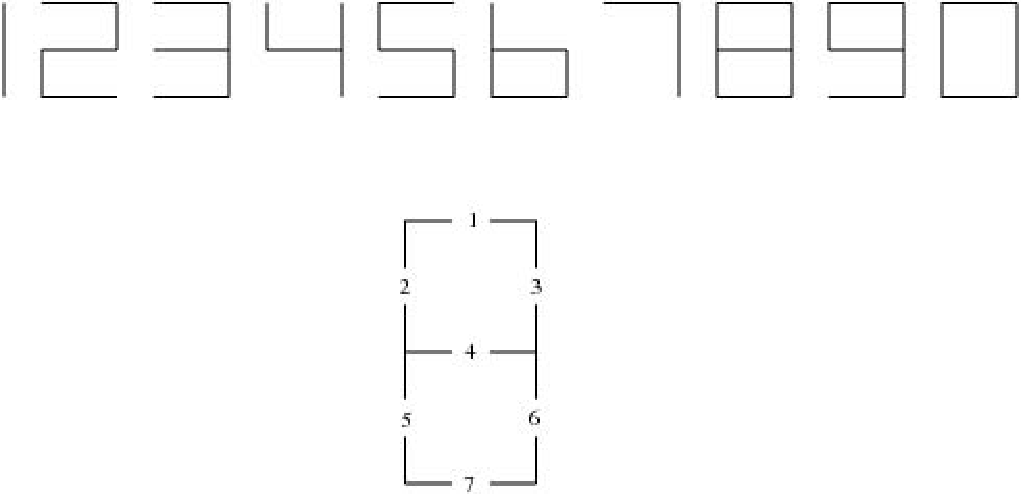
\includegraphics[width=3in]{Chp9_4.pdf}
\end{figure}

}



%%%--------------------------------------------------------------------

\frame {

\frametitle{}

\begin{table}
\centering
\begin{tabular}{c|ccccccc}
\hline
Digit & $x_{\cdot 1}$ & $x_{\cdot 2}$ & $x_{\cdot 3}$ & $x_{\cdot 4}$ & $x_{\cdot 5}$ & $x_{\cdot 6}$ & $x_{\cdot 7}$ \\
\hline
1 & 0 & 0 & 1 & 0 & 0 & 1 & 0 \\
2 & 1 & 0 & 1 & 1 & 1 & 0 & 1 \\
3 & 1 & 0 & 1 & 1 & 0 & 1 & 1 \\
4 & 0 & 1 & 1 & 1 & 0 & 1 & 0 \\
5 & 1 & 1 & 0 & 1 & 0 & 1 & 1 \\
6 & 1 & 1 & 0 & 1 & 1 & 1 & 1 \\ 
7 & 1 & 0 & 1 & 0 & 0 & 1 & 0 \\
8 & 1 & 1 & 1 & 1 & 1 & 1 & 1 \\
9 & 1 & 1 & 1 & 1 & 0 & 1 & 1 \\
0 & 1 & 1 & 1 & 0 & 1 & 1 & 1 \\
\hline
\end{tabular}
\end{table}

}



%%%--------------------------------------------------------------------

\frame {

\frametitle{}

\begin{itemize}
\item The data for the example are generated by a malfunctioning calculator
\item Each of the seven lights has probability 0.1 of being in the wrong state independently
\item The training set contains 200 samples generated according to the specified distribution
\end{itemize}

}



%%%--------------------------------------------------------------------

\frame {

\frametitle{ }

\begin{figure}
\centering
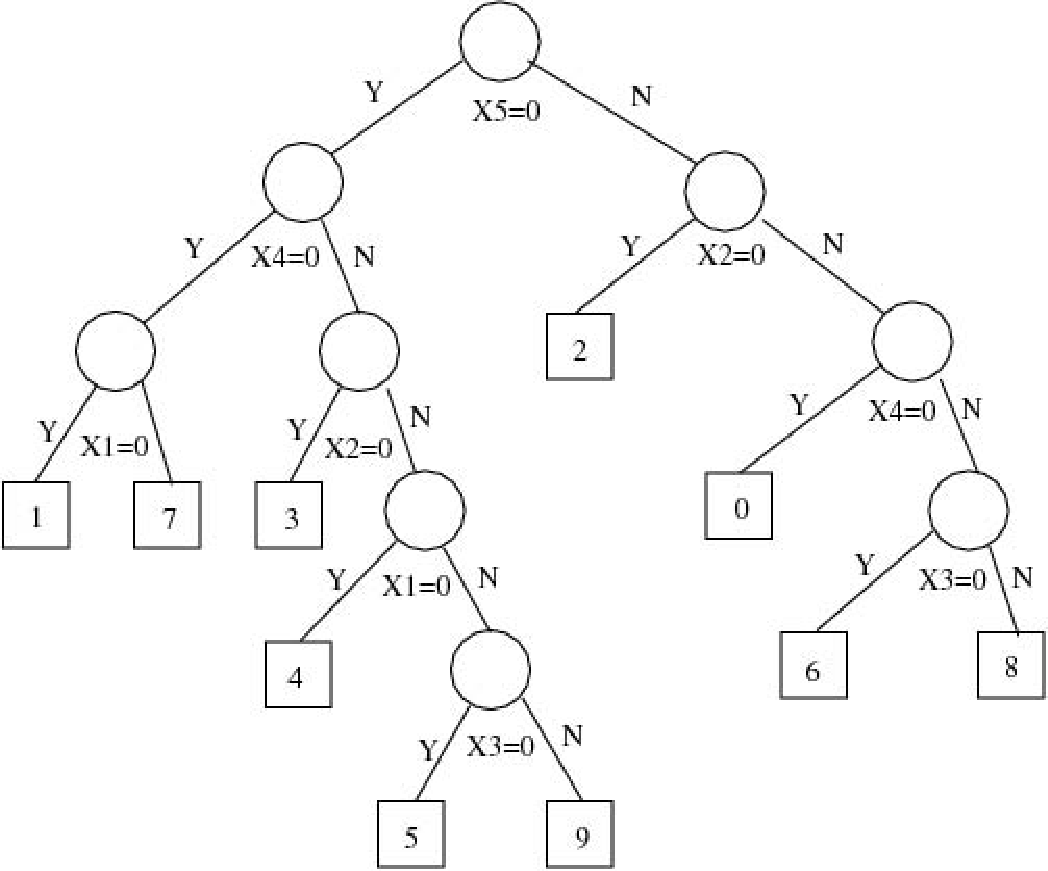
\includegraphics[width=4in]{Chp9_5.pdf}
\end{figure}

}



%%%--------------------------------------------------------------------

\frame {

\frametitle{Right-sized trees}


\begin{itemize}
\item Denote the misclassification error of a tree $T$ by $R(T)$, then
$$
R(T) = \sum_{t \in \tilde T} p(t) i(t),
$$
where $p(t) = |t|/n$ is the proportion of observations in node $t$, and $i(t)$ is defined by the misclassification error
\item $R(T)$ is biased downward, because
$$
p(t) i(t) \geq p(t_L) i(t_L) + p(t_R) i(t_R),
$$
thus the larger the tree is, the smaller the misclassification error (\structure{overfitting!})
\end{itemize}


}




%%%--------------------------------------------------------------------

\frame {

\frametitle{Digit recognition example: cont'd}


\begin{table}
\centering
\begin{tabular}{ccc}
\hline
No. Terminal Nodes & $R(T)$ &  $R^{ts}(T)$ \\
\hline
71 & .00 & .42 \\
63 & .00 & .40 \\
58 & .03 & .39 \\
40 & .10 & .32 \\
34 & .12 & .32 \\
19 & .29 & .31 \\
10 & .29 & .30 \\
9 & .32 & .34 \\
7 & .41 & .47 \\
6 & .46 & .54 \\
5 & .53 & .61 \\
2 & .75 & .82 \\
1 & .86 & .91 \\
\hline
\end{tabular}
\end{table}
Second column: training error;
Third column: test error.
}



%%%--------------------------------------------------------------------

\frame {

\frametitle{Pruning}


\begin{itemize}
\item Grow a very large tree $T_{max}$
\begin{enumerate}
\item Until all terminal nodes are pure (contain only one class) or contain only identical measurement vectors
\item When the number of data in each terminal node is no greater than a certain threshold
\item As long as the tree is sufficiently large
%the size of the initial tree is not critical
\end{enumerate}

\vspace{5mm}
\item A ``selective" pruning procedure is needed
\begin{enumerate}
\item The pruning is optimal in a certain sense
\item The search for different ways of pruning should be of manageable computational load
\end{enumerate}
\end{itemize}


}



%%%--------------------------------------------------------------------

\frame {

\frametitle{Minimal cost pruning}

For any subtree $T$ of $T_{max}$, define its cost function as
$$
R_{\lambda}(T)=R(T) + \lambda |\widetilde T|,
$$
where $\lambda$ is a tuning parameter. For each $\lambda$, solve
$$
T(\lambda) = \argmin_{T} R_{\lambda}(T)
$$

Remarks:
\begin{itemize}
\item To optimally determine $\lambda$, a model selection criterion such as cross validation can be employed
\item To search for the pruning branch, many technique has been proposed, such as the weakest-link cutting
\end{itemize}


}



%%%--------------------------------------------------------------------

\frame {

\frametitle{Advantages of the tree-structured approach}

\begin{itemize}
\item Handles both categorical and ordered variables in a simple and natural way
\item Automatic stepwise variable selection and complexity reduction
\item It provides an estimate of conditional class probability
\item It is invariant under all monotone transformations of individual ordered variables
\item Robust to outliers and misclassified points in the training set
\item {\bf Easy to interpret}
\end{itemize}

}



%%%--------------------------------------------------------------------

\frame {

\frametitle{Issues}

\begin{itemize}
\item Learning an optimal decision tree is NP-complete.
Categorical covariate with $q$ classes produces $2^q-1$ possible splits
\begin{itemize}
\item Simplification is possible for binary classification with Gini index or cross entropy and regression with squared error loss
\item But it is unclear for multiclass classification (digit recognition example)
\end{itemize}
\item Cost-sensitive (non-standard) classification with unequal misclassification costs
\item Splits based on combined covariates
\item Lack of smoothness (blockwise constant)
\item 
 \textcolor{red}{High variance, constructed tree is very sensitive to sample}

Trees can be very non-robust.A small change in the training data can result in a large change in the tree
\end{itemize}

}

\frame{{From Tree to Ensemble of trees}

Some techniques, often called ensemble methods, construct more than one decision tree:
\begin{enumerate}
\item 
{\bf Boosted trees}:  Incrementally building an ensemble by training each new instance to emphasize the training instances previously mis-modeled. A typical example is AdaBoost. These can be used for regression-type and classification-type problems.

We shall have one chapter focusing on boosting algorithms.

\item
{\bf Bootstrap aggregated (or bagged) decision trees}:  an early ensemble method, builds multiple decision trees by repeatedly resampling training data with replacement, and voting the trees for a consensus prediction.

\begin{itemize}
\item A {\bf random forest} classifier is a specific type of bootstrap aggregating
\end{itemize}
\end{enumerate}
}



%%%--------------------------------------------------------------------

\frame {

\frametitle{Bagging (bootstrap aggregation)}

{\it Bagging} is a technique to reduce the variance of an estimated prediction function.  
\begin{enumerate}
\item Draw  $B$ bootstrap samples
\footnote{these samples are
randomly drawn from the 
original dataset ${\cal D}=\{  (x_i,y_i)\}$ with replacement} $(x_1^{*b},y_1^{*b}),\ldots,(x_n^{*b},y_n^{*b})$; $b=1,\ldots,B$
\item For each bootstrap sample, fit the tree model $\hat f^{*b}(x)$
\item The bagging estimate is
$$
\hat f_{bag}(x) = \left \{ \begin{array}{l}
                           B^{-1} \sum_{b=1}^B \hat f^{*b}(x),~\mbox{for regression/classification}; \\
                           \mbox{mode}(\hat f^{*1}(x),\ldots,\hat f^{*B}(x)),~\mbox{for classification}
                           \end{array}
                  \right .
$$
\end{enumerate}

}



%%%--------------------------------------------------------------------

\frame {

\frametitle{Why it works: some intuitions}

\begin{itemize}
\item For regression, pretend we draw bootstrap samples from the true distribution rather than
the training set ${\cal D}$ (so \textcolor{red}{independent}), 
    $$
    E_{X,Y}(Y-\hat f(X))^2 \geq E(Y- \hat f_{bag}(X))^2,
    $$
    as one could see that $\hat f_{bag}(x) = E_{{\cal T}}(\hat f(x))$
\item For classification, $\hat f_{bag}(x) \neq E_{{\cal T}}(\hat f(x))$ and hence that the above inequality does not hold
\begin{itemize}
\item ``wisdom of crowds": the collective knowledge of a diverse and \textcolor{red}{independent} body of people exceeds the knowledge of any single individual
\item Two heads are better than one
\end{itemize}
\end{itemize}

}




%%%--------------------------------------------------------------------

\frame {

\frametitle{Random forest}

Random forest is similar to bagging, but different as it averages {\it de-correlated} trees
by introducing 
{\it additional randomness}
in each tree $\hat{f}^{*,b}(x)$
by using  random subsets of features

\vspace{0.5cm}
\begin{enumerate}
\item Draw bootstrap samples $(x_1^{*b},y_1^{*b}),\ldots,(x_n^{*b},y_n^{*b})$
\item For each bootstrap sample, grow a tree by repeating:
\begin{enumerate}[a.]
\item \textcolor{red}{randomly select a subset of the $p$ covariates}
\item pick the best split among the chosen subset
\item split the node
\end{enumerate}
\item The random forest estimate is constructed similarly as in bagging (average for regression, and majority vote for classification)
\end{enumerate}

}



%%%--------------------------------------------------------------------

\frame {

\frametitle{Why it works: some intuitions}

\begin{itemize}
\item In bagging, the bootstrap trees are correlated, and correlation limits the benefit of averaging
\item Averaging $B$ 
random variables with variance $\sigma^2$ and correlation $\rho$ yields the variance\footnote{
the proof is an exercise}
    $$
    \rho \sigma^2 + \frac{1-\rho}{B} \sigma^2
    =\rho \sigma^2 (1-\frac{1}{B}) + \frac{\sigma^2}{B}
    $$ 
\item In random forest, the correlation is reduced by selection of covariates in growing trees
\item The price it has to pay is the increment of bias and variance, which, fortunately, is usually small
\item \href{https://www.stat.berkeley.edu/~breiman/randomforest2001.pdf}
{Breiman 2001 paper}
\end{itemize}

}

\frame{{Random Forest: pro and con}
Advantage:
\begin{enumerate}
\item  flexible, nonlinear decision boundary 
\item  easy to implement;  favourite of CS programmers 
\item easy to use and interpret
\item it can be used for both regression and classification tasks
\item not seen to overfit easily
\end{enumerate}

Limits:
\begin{enumerate}
\item a large number of trees can make the algorithm to slow and ineffective for real-time predictions.

\medskip {\it Committee make any decision very slowly.}
\item High dimension and small/unbalanced samples?
\end{enumerate}


}



%%%--------------------------------------------------------------------

\frame {

\frametitle{Additional readings and resource}

Breiman, L. (2001). Random forests. {\it Mach. Learn.}, {\bf 45}, 5-32.

\bigskip
Biau, G., Devroye, L. and Lugosi, G. (2008). Consistency of random forests and other averaging classifiers. {\it J. Mach. Learn. Res.}, {\bf 9}, 2039-2057.


\bigskip

\href{https://arxiv.org/pdf/0811.3619.pdf}{Random Forests: some methodological insights, 2008}

\bigskip 
\href{https://towardsdatascience.com/an-implementation-and-explanation-of-the-random-forest-in-python-77bf308a9b76}{An Implementation and Explanation of the Random Forest in Python
}

\bigskip 
\href{https://en.wikipedia.org/wiki/Random_forest}
{Wikipedia of Random Forest}
}


\end{document}
